\documentclass{article}

\usepackage{enumerate}
\usepackage{amssymb}
\usepackage{amsmath}
\usepackage{algorithm}
\usepackage{physics}
\usepackage{listings}
\usepackage[noend]{algpseudocode}
\usepackage{graphicx}

\graphicspath{ {./} }

\topmargin=-0.45in
\evensidemargin=0in
\oddsidemargin=0in
\textwidth=6.5in
\textheight=9.0in
\headsep=0.25in

\title{Chem 195: Problem Set 11}
\author{Michael Stephen Chen}


\begin{document}
\maketitle
\pagebreak

\section*{Problem 1}
\begin{enumerate}[i.]
  \item See \textit{hard\_disks\_p.m}
  \item Below is a plot depicting $g(r) vs. r$ for a fixed density (0.7) hard disk simulation
    \begin{center}
      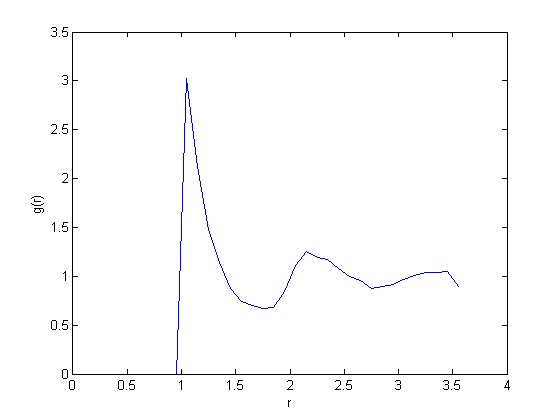
\includegraphics[scale=0.5]{Density/1ii}
    \end{center}

  \item A representative plot of the particles at equilibrium is displayed below
    \begin{center}
      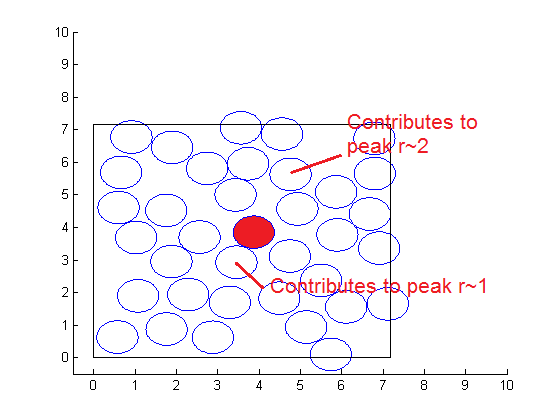
\includegraphics[scale=0.5]{Density/1iii}
    \end{center}

  \item Below is a plot depicting $g(r) vs. r$ for various densities
    \begin{center}
      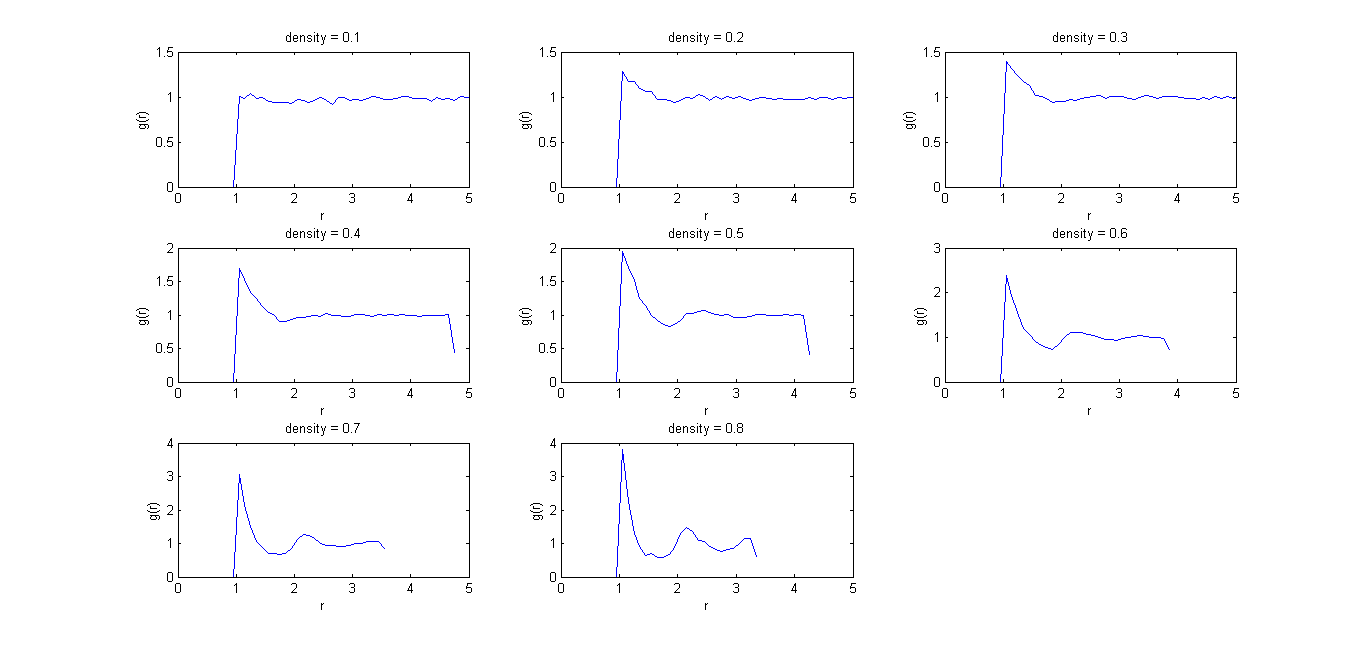
\includegraphics[scale=0.5]{Density/1iv}
    \end{center}

    The table below presents our simulated values for $g(\sigma +)$ for various densities
    \begin{center}
      $\begin{array}{c|c}
        Density & g(sigma+) \\ \hline
        0.1 & 1.010 \\
        0.2 & 1.279 \\
        0.3 & 1.397 \\
        0.4 & 1.696 \\
        0.5 & 1.952 \\
        0.6 & 2.389 \\
        0.7 & 3.051 \\
        0.8 & 3.811 \\
      \end{array}$
    \end{center}

  \item Below is a plot of the fluid pressure as a function of density
    \begin{center}
      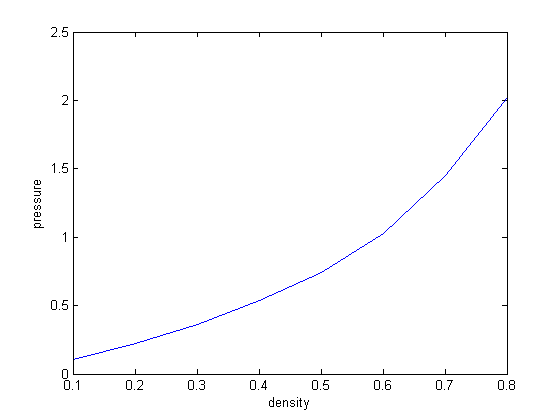
\includegraphics[scale=0.5]{Density/1v}
    \end{center}

  \item Using the constant pressure MC simulation we obtain the following results:
    \begin{center}
      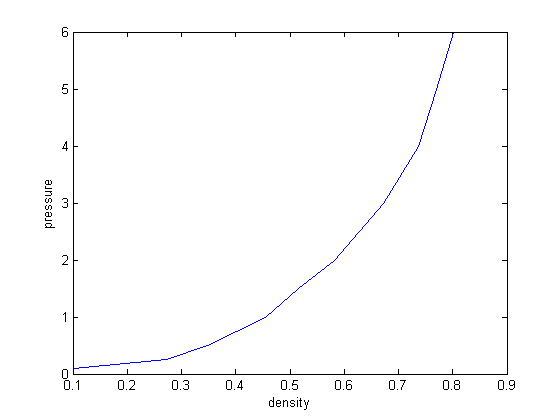
\includegraphics[scale=0.5]{Pressure/1vi}
    \end{center}

    Comparing this plot to the plot from part (v) we see that qualitatively they look similar (both upward curves). However the constant-pressure results grow considerably faster (pressure v. density).

  \item At higher pressures we observe a phase transition
    \begin{center}
      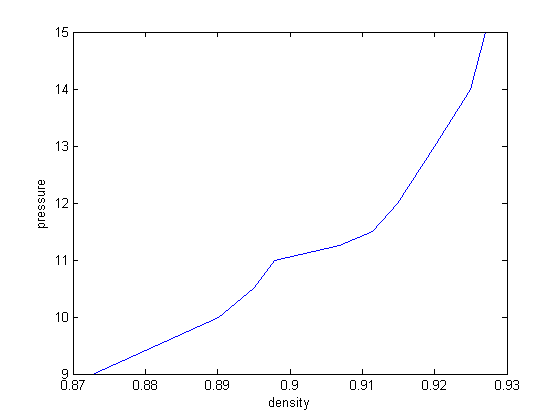
\includegraphics[scale=0.5]{Pressure/1vii}
    \end{center}
    
    The relatively flat region beginning at roughly $p^*=11$ is representative of the system undergoing a phase transition (because volume is constant during a phase transition and density is inversely proportional to volume). Using the data points in the linear region, linear regression was used to determine a best-fit line relating pressure to average density:
    $$P = 0.027\rho + 0.6016$$

\end{enumerate}


\section*{Problem 2}
\begin{enumerate}[i.]
  \item Given that we are using periodic boundary conditions, if we did not truncate at some reasonable distance $r_{cut} \leq L/2$ where L is our box width/height then we run into the possibility of double/(perhaps more?) counting interactions. So we impose an $r_{cut}$ to maintain minimum-image convention. However in the case of our simulation where we iterate over all particles only once per iteration, this is implicitly taken care of.

  \item See \textit{LJPotential.m}. A plot of my results is displayed below:
    \begin{center}
      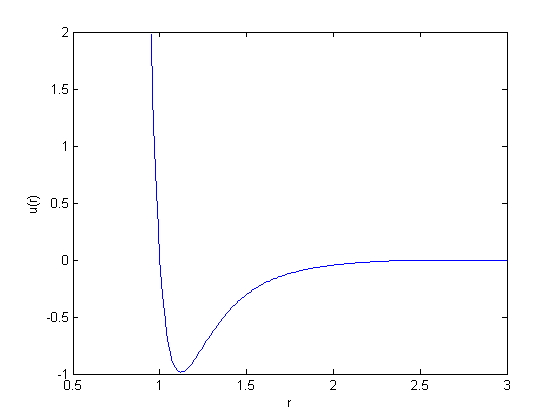
\includegraphics[scale=0.5]{LJ/2ii}
    \end{center}

  \item See \textit{LJPotentialTotal.m}.

  \item A plot of my results is displayed below
    \begin{center}
      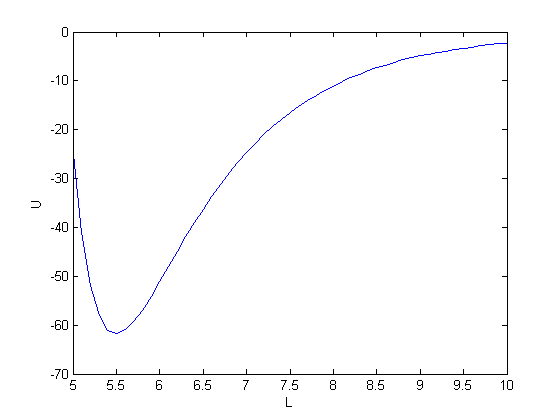
\includegraphics[scale=0.5]{LJ/2iv}
    \end{center}

  \item See \textit{prob2.m}. I found $\Delta U = -0.05$. When I displayed a different particle in the same way, I got the same exact energy change values. This makes sense because we are using periodic boundary conditions, making it so that it is indistinguishable whether we displace \#1 or \#2 from the perfect lattice. I also found that displacing \#1 in a different direction (while keeping the same magnitude) resulted in the same energy change as well. Which seems to make sense because the potential is only a function of the distance (not direction) and by displacing \#1, we make \#1 closer to some particles and farther from others in such a way that the effects cancel.

  \item See \textit{LJSimulation.m}

  \item My simulation result is below
    \begin{center}
      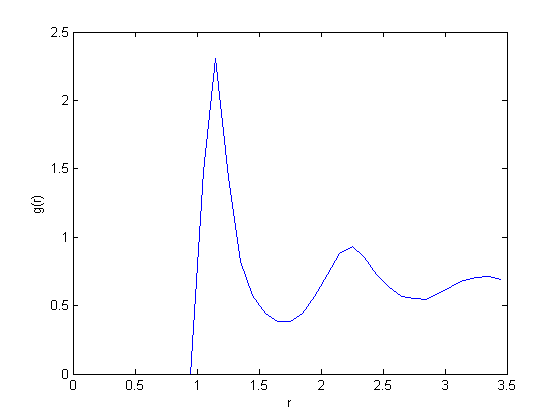
\includegraphics[scale=0.5]{LJ/2vii}
    \end{center}

    Qualitatively the this is very similar to the hard disk result, with the same number of peaks that have the same shape. The biggest differnece is that the LJ plot has lower magnitudes for the range we plotted as compared to the hard disk simulation. 
    
  \item A histogram for the potential energies is displayed below
    \begin{center}
      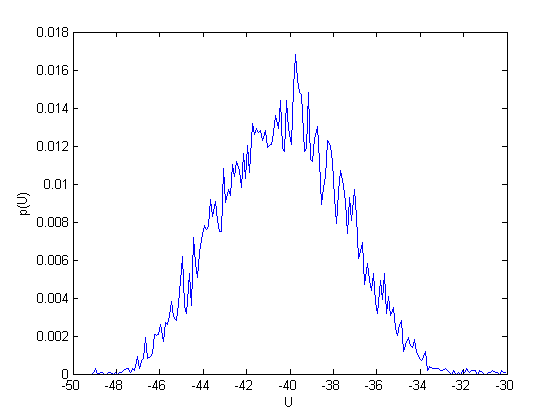
\includegraphics[scale=0.5]{LJ/2viii}
    \end{center}

\end{enumerate}

\end{document}
